% Importado desde: 2026-03-28_SSH_a_Dirac_1D.tex
\chapter{Derivacion Pedagogica: --- Del modelo SSH a una ecuacion de Dirac en \(1+1\)}
\label{ch:ssh-a-dirac-1d}






% verified-by: validators/ssh.py::test_ssh_squared
% verified-by: validators/ssh.py::test_ssh_gap_closes
% verified-by: validators/ssh.py::test_ssh_linearization

\section{Objetivo}

El modelo de Su--Schrieffer--Heeger (SSH) es el ejemplo unidimensional correcto para introducir una estructura espinorial efectiva en una red discreta. Su importancia dentro del programa de investigación es muy concreta:

\begin{enumerate}[leftmargin=*]
  \item tiene dos sitios por celda unitaria;
  \item el Hamiltoniano vive naturalmente en un espacio de dos componentes;
  \item el cierre del gap se controla con un parámetro;
  \item al linealizar cerca del punto crítico aparece un Hamiltoniano tipo Dirac en \(1+1\).
\end{enumerate}

En este documento vamos a derivar eso paso a paso, con cuentas intermedias y figuras, para dejar fijo el primer peldaño de la escalera conceptual del proyecto.

\section{La idea física del modelo SSH}

El modelo describe una cadena unidimensional con dos sitios por celda unitaria, que llamaremos \(A\) y \(B\). Los acoplos entre vecinos alternan entre dos valores:
\begin{equation}
t_1 \quad \text{e} \quad t_2.
\end{equation}

Esa alternancia es exactamente lo que permite abrir o cerrar un gap. Cuando \(t_1\neq t_2\), el sistema está gapped. Cuando \(t_1=t_2\), las bandas se tocan en el borde de la zona de Brillouin, y la teoría efectiva se vuelve de tipo Dirac.

\begin{figure}[ht]
\centering
\begin{tikzpicture}[>=Latex,scale=1.2]
  \foreach \x in {0,2,4,6}
    \fill[blue!70] (\x,0) circle (2.2pt);
  \foreach \x in {1,3,5,7}
    \fill[orange!85!black] (\x,0) circle (2.2pt);

  \foreach \x/\lab in {0/A_n,2/A_{n+1},4/A_{n+2}}
    \node[above] at (\x,0) {\small $\lab$};
  \foreach \x/\lab in {1/B_n,3/B_{n+1},5/B_{n+2}}
    \node[above] at (\x,0) {\small $\lab$};

  \draw[very thick] (0,0)--(1,0);
  \draw[very thick,dashed] (1,0)--(2,0);
  \draw[very thick] (2,0)--(3,0);
  \draw[very thick,dashed] (3,0)--(4,0);
  \draw[very thick] (4,0)--(5,0);
  \draw[very thick,dashed] (5,0)--(6,0);
  \draw[very thick] (6,0)--(7,0);

  \node[below] at (0.5,0) {$t_1$};
  \node[below] at (1.5,0) {$t_2$};
  \node[below] at (2.5,0) {$t_1$};
  \node[below] at (3.5,0) {$t_2$};
  \node[below] at (4.5,0) {$t_1$};
  \node[below] at (5.5,0) {$t_2$};

  \draw[decorate,decoration={brace,amplitude=5pt}] (-0.05,-0.55) -- (1.05,-0.55);
  \node[below=7pt] at (0.5,-0.55) {\small celda \(n\)};
  \draw[decorate,decoration={brace,amplitude=5pt}] (1.95,-0.55) -- (3.05,-0.55);
  \node[below=7pt] at (2.5,-0.55) {\small celda \(n+1\)};
\end{tikzpicture}
\caption{Cadena SSH. Cada celda unitaria contiene dos sitios, \(A\) y \(B\). El acoplo intracelda es \(t_1\) y el acoplo interceldas es \(t_2\).}
\label{c01:fig:ssh-chain}
\end{figure}

\section{Hamiltoniano tight-binding}

\subsection{Hamiltoniano en espacio real}

Denotemos por \(a_n^\dagger\) y \(b_n^\dagger\) los operadores de creación en los sitios \(A_n\) y \(B_n\). El Hamiltoniano SSH es
\begin{equation}
H =
\sum_n \left(
t_1\, a_n^\dagger b_n
+ t_2\, a_{n+1}^\dagger b_n
+ \text{h.c.}
\right).
\label{c01:eq:ssh-real}
\end{equation}

Su lectura física es directa:

\begin{enumerate}[leftmargin=*]
  \item \(t_1\) conecta \(A_n\) con \(B_n\) dentro de la misma celda;
  \item \(t_2\) conecta \(B_n\) con \(A_{n+1}\) entre celdas vecinas.
\end{enumerate}

\subsection{Por qué aparecen dos componentes}

Como hay dos sitios por celda unitaria, la función de onda de Bloch debe tener dos componentes:
\begin{equation}
\Psi_k =
\begin{pmatrix}
\psi_A(k)\\
\psi_B(k)
\end{pmatrix}.
\end{equation}

Eso es el análogo unidimensional del pseudospín de subred que luego aparece en grafeno. No es espín real; es el espacio interno \(A/B\) de la cadena.

\section{Paso al espacio recíproco}

\subsection{Transformada de Fourier}

Tomamos
\begin{equation}
a_n=\frac{1}{\sqrt{N}}\sum_k \ee^{\ii k n a} a_k,
\qquad
b_n=\frac{1}{\sqrt{N}}\sum_k \ee^{\ii k n a} b_k,
\label{c01:eq:ssh-fourier}
\end{equation}
donde \(a\) es la longitud de la celda y \(N\) el número de celdas.

Sustituimos \eqref{c01:eq:ssh-fourier} en \eqref{c01:eq:ssh-real}. El término intracelda queda
\begin{equation}
\sum_n t_1 a_n^\dagger b_n
=
t_1 \sum_k a_k^\dagger b_k,
\end{equation}
mientras que el término interceldas produce un factor de fase:
\begin{equation}
\sum_n t_2 a_{n+1}^\dagger b_n
=
t_2 \sum_k \ee^{-\ii k a} a_k^\dagger b_k.
\end{equation}

Por tanto,
\begin{equation}
H=\sum_k
\begin{pmatrix}
a_k^\dagger & b_k^\dagger
\end{pmatrix}
H(k)
\begin{pmatrix}
a_k\\
b_k
\end{pmatrix},
\end{equation}
con
\begin{equation}
H(k)=
\begin{pmatrix}
0 & t_1+t_2\ee^{-\ii k a}\\
t_1+t_2\ee^{\ii k a} & 0
\end{pmatrix}.
\label{c01:eq:ssh-bloch}
\end{equation}

\subsection{Escritura con matrices de Pauli}

Separando partes real e imaginaria,
\begin{equation}
t_1+t_2\ee^{-\ii ka}
=
t_1+t_2\cos(ka)-\ii t_2\sin(ka).
\end{equation}

Entonces el Hamiltoniano se puede escribir como
\begin{equation}
H(k)= d_x(k)\sigma_x + d_y(k)\sigma_y,
\end{equation}
con
\begin{equation}
d_x(k)=t_1+t_2\cos(ka),
\qquad
d_y(k)=t_2\sin(ka).
\label{c01:eq:ssh-dxdy}
\end{equation}

Dependiendo de la convención, el signo delante de \(\sigma_y\) puede cambiar. La física no cambia.

\section{Bandas y cierre del gap}

\subsection{Autovalores}

Como el Hamiltoniano es de la forma \(H=\bm{d}\cdot\bm{\sigma}\), los autovalores son
\begin{equation}
E_\pm(k)=\pm \sqrt{d_x(k)^2+d_y(k)^2}.
\end{equation}

Sustituyendo \eqref{c01:eq:ssh-dxdy},
\begin{equation}
E_\pm(k)=
\pm \sqrt{(t_1+t_2\cos ka)^2+t_2^2\sin^2 ka}.
\end{equation}

Agrupando,
\begin{equation}
E_\pm(k)=
\pm \sqrt{t_1^2+t_2^2+2t_1 t_2 \cos(ka)}.
\label{c01:eq:ssh-dispersion}
\end{equation}

\subsection{Condición de cierre del gap}

Para que las bandas se toquen, debe ocurrir
\begin{equation}
d_x(k)=0,
\qquad
d_y(k)=0.
\end{equation}

La segunda ecuación exige
\begin{equation}
\sin(ka)=0
\quad \Longrightarrow \quad
ka=0,\pi.
\end{equation}

Probamos esos dos casos:

\begin{enumerate}[leftmargin=*]
  \item si \(ka=0\), entonces \(d_x=t_1+t_2\), que no se anula salvo en el caso trivial \(t_1=-t_2\);
  \item si \(ka=\pi\), entonces \(d_x=t_1-t_2\).
\end{enumerate}

Luego el cierre del gap ocurre en
\begin{equation}
k_0=\frac{\pi}{a},
\qquad
t_1=t_2.
\label{c01:eq:ssh-critical}
\end{equation}

Ese es el punto crítico del modelo SSH.

\begin{figure}[ht]
\centering
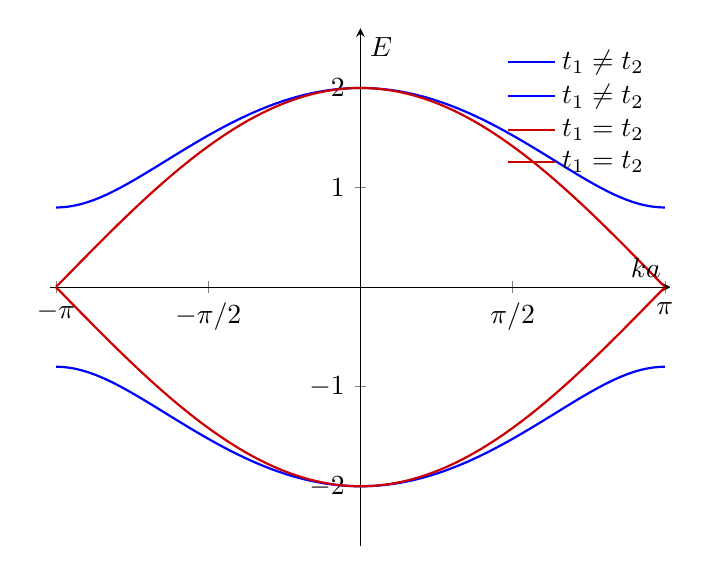
\begin{tikzpicture}
\begin{axis}[
  width=0.78\textwidth,
  xlabel={$ka$},
  ylabel={$E$},
  xmin=-3.2,xmax=3.2,
  ymin=-2.6,ymax=2.6,
  axis lines=middle,
  xtick={-3.1416,-1.5708,0,1.5708,3.1416},
  xticklabels={$-\pi$,$-\pi/2$,$0$,$\pi/2$,$\pi$},
  samples=300,
  domain=-3.1416:3.1416,
  legend style={draw=none,fill=none,at={(0.98,0.98)},anchor=north east}
]
\addplot[thick,blue] {sqrt(0.6^2+1.4^2+2*0.6*1.4*cos(deg(x)))};
\addplot[thick,blue] {-sqrt(0.6^2+1.4^2+2*0.6*1.4*cos(deg(x)))};
\addplot[thick,red!80!black] {sqrt(1+1+2*cos(deg(x)))};
\addplot[thick,red!80!black] {-sqrt(1+1+2*cos(deg(x)))};
\legend{\(t_1\neq t_2\),\(t_1\neq t_2\),\(t_1=t_2\),\(t_1=t_2\)}
\end{axis}
\end{tikzpicture}
\caption{Dispersión del modelo SSH. En azul, el caso gapped \(t_1\neq t_2\). En rojo, el caso crítico \(t_1=t_2\), donde el gap se cierra en \(ka=\pi\).}
\label{c01:fig:ssh-disp}
\end{figure}

\section{Linealización alrededor del punto crítico}

\subsection{Expansión alrededor de k0 = pi/a}

Escribimos
\begin{equation}
k = \frac{\pi}{a}+q,
\qquad |q a|\ll 1.
\end{equation}

Entonces
\begin{align}
\cos(ka)
&=
\cos(\pi+qa)
=
-\cos(qa)
\approx -1,
\\
\sin(ka)
&=
\sin(\pi+qa)
=
-\sin(qa)
\approx -qa.
\end{align}

Sustituyendo en \eqref{c01:eq:ssh-dxdy},
\begin{align}
d_x(k)
&\approx t_1-t_2,
\\
d_y(k)
&\approx -t_2\, a\, q.
\end{align}

Por tanto, cerca del punto crítico:
\begin{equation}
H(q)\approx (t_1-t_2)\sigma_x - t_2 a q\,\sigma_y.
\label{c01:eq:ssh-linear}
\end{equation}

\subsection{Caso exactamente crítico}

Si \(t_1=t_2=t\), el primer término desaparece y queda
\begin{equation}
H_{\text{crit}}(q)\approx - t a q\, \sigma_y.
\label{c01:eq:ssh-critical-linear}
\end{equation}

Eso es ya un Hamiltoniano lineal en el momento, exactamente lo que esperamos de una teoría de Dirac sin masa en \(1+1\).

\subsection{Interpretación del término t1 - t2}

Definimos
\begin{equation}
m \equiv t_1-t_2,
\qquad
v \equiv t a.
\end{equation}

Entonces \eqref{c01:eq:ssh-linear} se escribe como
\begin{equation}
H(q)\approx m\,\sigma_x - v q\,\sigma_y.
\label{c01:eq:ssh-massive-dirac}
\end{equation}

Esta es la forma estándar de un Hamiltoniano de Dirac masivo en \(1D\): un término lineal en el momento más un término de masa controlable.

\section{Relación con la ecuación de Dirac}

\subsection{Estructura relativista efectiva}

Si promovemos \(q\to -\ii \partial_x\), la ecuación efectiva toma la forma
\begin{equation}
\ii \partial_t \Psi =
\left(
m\,\sigma_x + \ii v\,\sigma_y \partial_x
\right)\Psi.
\label{c01:eq:ssh-dirac-real}
\end{equation}

Con una redefinición conveniente de matrices, esto es equivalente a una ecuación de Dirac en \(1+1\):
\begin{equation}
\left(
\ii \gamma^\mu \partial_\mu - m
\right)\Psi=0.
\end{equation}

Lo importante aquí no es la representación específica de las matrices gamma, sino el hecho estructural:

\begin{enumerate}[leftmargin=*]
  \item el grado de libertad de subred produce un espinor de dos componentes;
  \item la linealización del Hamiltoniano produce un operador de primer orden;
  \item la diferencia \(t_1-t_2\) actúa exactamente como una masa efectiva.
\end{enumerate}

\subsection{Espectro efectivo}

Del Hamiltoniano \eqref{c01:eq:ssh-massive-dirac}, el espectro es
\begin{equation}
E_\pm(q)=\pm \sqrt{m^2+v^2 q^2}.
\label{c01:eq:ssh-effective-disp}
\end{equation}

Si \(m=0\), obtenemos una dispersión lineal gapless. Si \(m\neq 0\), se abre un gap de tamaño
\begin{equation}
\Delta = 2|m| = 2|t_1-t_2|.
\end{equation}

\begin{figure}[ht]
\centering
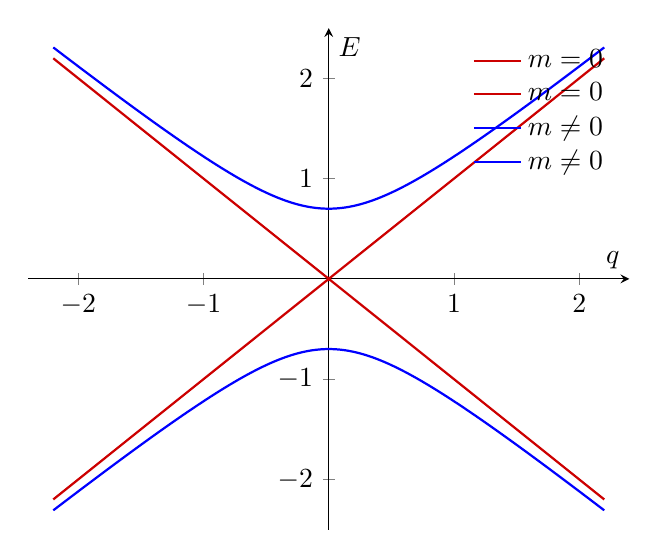
\begin{tikzpicture}
\begin{axis}[
  width=0.76\textwidth,
  xlabel={$q$},
  ylabel={$E$},
  xmin=-2.4,xmax=2.4,
  ymin=-2.5,ymax=2.5,
  axis lines=middle,
  samples=250,
  domain=-2.2:2.2,
  legend style={draw=none,fill=none,at={(0.98,0.98)},anchor=north east}
]
\addplot[thick,red!80!black] {abs(x)};
\addplot[thick,red!80!black] {-abs(x)};
\addplot[thick,blue] {sqrt(0.7^2+x^2)};
\addplot[thick,blue] {-sqrt(0.7^2+x^2)};
\legend{\(m=0\),\(m=0\),\(m\neq 0\),\(m\neq 0\)}
\end{axis}
\end{tikzpicture}
\caption{Dispersión efectiva del modelo linealizado. El caso crítico \(m=0\) produce un cono lineal en \(1D\); el caso \(m\neq 0\) abre una brecha.}
\label{c01:fig:ssh-effective}
\end{figure}

\section{Interpretación topológica mínima}

Aunque aquí estamos usando el modelo sobre todo como ejemplo de Dirac emergente, el SSH también enseña una lección topológica importante. Los dos regímenes:
\begin{equation}
t_1>t_2
\qquad \text{y} \qquad
t_2>t_1
\end{equation}
no son simplemente dos versiones cuantitativas del mismo sistema; corresponden a fases topológicas distintas.

El punto crítico \(t_1=t_2\) separa esas dos fases. En el lenguaje efectivo, eso se refleja en el cambio de signo de la masa:
\begin{equation}
m=t_1-t_2.
\end{equation}

Esto es pedagógicamente muy valioso para el proyecto, porque más adelante en grafeno, y todavía más en Dirac/Weyl 3D, veremos que cambiar el signo de un término de masa o romper una simetría puede cambiar por completo la naturaleza de la fase.

\section{Qué enseña SSH para el proyecto}

El modelo SSH deja ya fijadas varias lecciones centrales:

\begin{enumerate}[leftmargin=*]
  \item una red discreta con estructura interna puede producir espinores efectivos;
  \item una teoría tipo Dirac emerge por linealización alrededor de un punto de cierre del gap;
  \item la masa efectiva se controla con un parámetro microscópico sencillo;
  \item una transición de fase puede leerse como cambio de signo del término de masa.
\end{enumerate}

En otras palabras: SSH es el laboratorio mínimo donde aparecen, en forma limpia, pseudospín, cierre del gap, masa efectiva y Dirac emergente.

\section{Mapa de la derivación}

\begin{figure}[ht]
\centering
\begin{tikzpicture}[
  node distance=8mm and 9mm,
  every node/.style={font=\small},
  box/.style={draw,rounded corners,thick,align=center,minimum width=3.2cm,minimum height=1cm,fill=blue!6},
  arr/.style={-{Latex[length=3mm]},thick}
]
  \node[box] (a) {Cadena con dos sitios\\ por celda \(A/B\)};
  \node[box, right=of a] (b) {Hamiltoniano SSH\\ \(t_1,t_2\)};
  \node[box, right=of b] (c) {Hamiltoniano de Bloch\\ \(H(k)\)};
  \node[box, below=of b] (d) {Cierre del gap\\ \(t_1=t_2,\; k=\pi/a\)};
  \node[box, left=of d] (e) {Linealización\\ \(k=\pi/a+q\)};
  \node[box, right=of d] (f) {Dirac 1D\\ \(H\approx m\sigma_x-vq\sigma_y\)};

  \draw[arr] (a) -- (b);
  \draw[arr] (b) -- (c);
  \draw[arr] (c) -- (d);
  \draw[arr] (d) -- (e);
  \draw[arr] (d) -- (f);
\end{tikzpicture}
\caption{Ruta conceptual del capítulo SSH.}
\label{c01:fig:ssh-roadmap}
\end{figure}

\section{Dónde encaja dentro del programa}

Este documento cumple exactamente el primer paso sugerido en tu programa:

\begin{enumerate}[leftmargin=*]
  \item reemplaza la cadena unidimensional simple por el ejemplo correcto, el SSH;
  \item muestra cómo aparece una estructura espinorial efectiva en \(1D\);
  \item introduce la masa efectiva de forma controlable;
  \item prepara el lenguaje que luego se reutiliza en grafeno y en modelos \(3D\).
\end{enumerate}

La secuencia del proyecto queda ahora mucho más ordenada:

\begin{enumerate}[leftmargin=*]
  \item SSH \(\rightarrow\) Dirac \(1+1\),
  \item grafeno \(\rightarrow\) Dirac \(2+1\),
  \item semimetales \(\rightarrow\) Dirac/Weyl en \(3D\),
  \item luego Nielsen--Ninomiya y, si conviene, tiempo discreto.
\end{enumerate}
